\documentclass[10pt]{exam}
\usepackage[phy]{template-for-exam}
\usepackage{mdframed,multirow,enumitem,silence,tikz,graphicx,multicol}
\WarningFilter{latex}{Label `question}
\WarningFilter{latex}{There were multiply-defined labels}
\usetikzlibrary{shadings,decorations.pathmorphing,arrows.meta,patterns}


\title{Designing a Measurement Lab}
\author{Rohrbach}
\date{\today}

\begin{document}
\maketitle

\vspace{-2em}
\begin{questions}
    \uplevel{\section*{Pre-Lab}}
  
    \question
      What can we measure on the different balls?  Make 
      a list of as many things as possible. 
      \vs[3]

    \question
      Identify each of the following (there may be more 
      than one):
      
      \begin{center}
        \begin{tabular}
          { m{.25\textwidth} | m{.3\textwidth}| m{.25\textwidth} } 
          Independent Variables & 
          Dependent Variables   & 
          Control Variables  \\[8em]
        \end{tabular}
      \end{center}
    
  
\end{questions}

\section*{Purpose}
Write down one sentence explainging the purpose of the lab that includes all the independent and dependent variable.
\vs[2]

\section*{Procedure}

Materials:

\begin{itemize}[topsep=0pt,itemsep=-1ex,partopsep=1ex,parsep=1ex]
  \item two different balls
  \item one meter stick
\end{itemize}


\noindent When you're ready to start the experiment:

\begin{enumerate}[topsep=0pt,itemsep=-1ex,partopsep=1ex,parsep=1ex]
  \item Drop the ball
  \item Stand back and watch how high the ball bounces
  \item Record the Data.
\end{enumerate}

\pagebreak

\section*{Data}



\def\cw{.15\textwidth}
\def\ch{1em}

\newcommand{\datatable}{
  \begin{center}
    \begin{tabular}
      {|*{5}{>{\centering\arraybackslash}m{\cw}|}}
      \hline
      \multirow{2}{\cw}
        {\centering Drop Height (cm)} & 
      \multicolumn{4}{c|}{Bounce Height (cm)} \\
      \cline{2-5}
      & Trial \#1 & Trial \#2 & Trial \#3 & Average \\
      \hline
      &&&&\\[\ch]
      \hline
      &&&&\\[\ch]
      \hline
      &&&&\\[\ch]
      \hline
      &&&&\\[\ch]
      \hline
      &&&&\\[\ch]
      \hline
    \end{tabular}
  \end{center}
}


\subsection*{Experiment \#1}

Constant(s): \fillin[][15em]

\datatable

\subsection*{Experiment \#2}

Constant(s): \fillin[][15em]

\datatable


\section*{Graphs}

Go to \texttt{www.desmos.com/calculator} to graph your data.

\begin{multicols}{2}

\begin{enumerate}[label=\alph*),topsep=0pt,itemsep=-1ex,partopsep=1ex,parsep=1ex]
  \item \label{table} Start by making a table by clicking the “+” icon at the top left.  You will need to create two separate tables.
  \item \label{wrench} Make sure to label the axes using the wrench icon at the right.
  \item \label{zoom} Zoom out so that you can see the whole graph and so that it fills the page.  You can do this using the ``Zoom Fit'' option , but be careful that your fit does not cut off one of the graphs
  \item \label{linear} Create best fit lines for each graph using the ``Linear Regression'' tool
  \item Copy a link to your graph using the export button and clicking ``Share a Snapshot''.  Paste this link on the appropriate place in Schoology.
\end{enumerate}

  \begin{tikzpicture}
    \node[anchor=north west] at (0,0) 
      {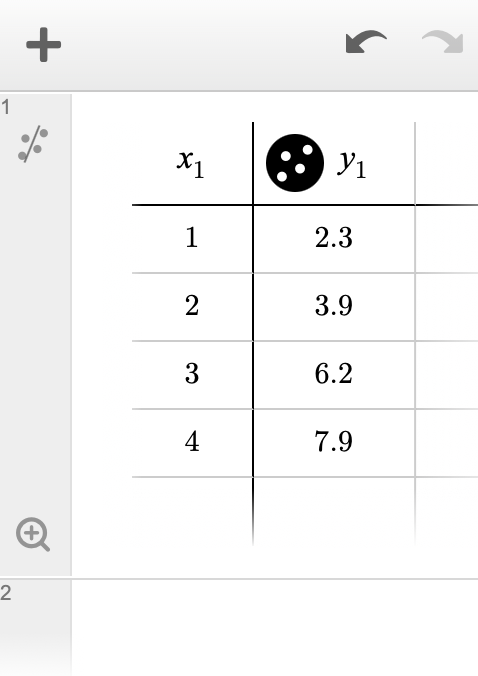
\includegraphics[width=3cm]{desmos1}};


    \node[anchor=north west] at (3.5,0) 
      {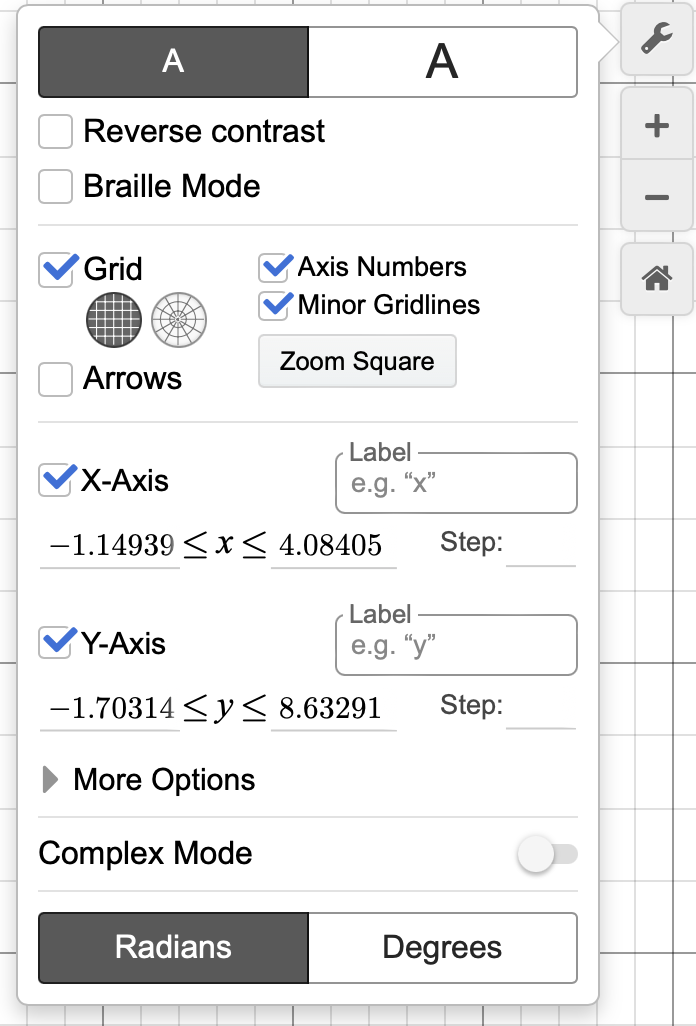
\includegraphics[width=3.5cm]{desmos2}};

        \draw (2,0) 
      node[fill=red!20,rounded corners] (table)
      {\ref{table} Create a table};
    \draw[red] (0.4,-.4) coordinate (a) circle (0.3);
    \draw[<-,red,very thick] (a) +(0.3,0) -- (table.south);

    \node[fill=blue!20,rounded corners] at (2.5,-1.5) (linear) {\ref{linear} Linear Regression};
    \draw[blue] (0.3,-1) coordinate (a) circle (0.3);
    \draw[<-,blue,very thick] (a) +(0.3,0) -- (linear.north);

    \node[fill=green!20,rounded corners] at (2,-2.5) (zoom) {\ref{zoom} Zoom Fit};
    \draw[green, ultra thick] (0.3,-3.5) coordinate (a) circle (0.3);
    \draw[<-,green,very thick] (a) +(0.3,0) -- (zoom.west);

    \node[fill=orange!20,rounded corners] at (4.5,-0.5) (wrench) {\ref{wrench} Axis Labels};
    \draw[orange, ultra thick] (6.9,-.3) coordinate (a) circle (0.3);
    \draw[<-,orange,very thick] (a) +(-0.3,0) -- (wrench.east);

    \draw[->,orange,very thick] (wrench.south) -- (5.2,-2.3);

    \draw[orange, ultra thick, rounded corners] (3.8,-2.3) rectangle ++(2.8,-0.5);
    \draw[orange, ultra thick, rounded corners] (3.8,-3.1) rectangle ++(2.8,-0.5);
  \end{tikzpicture}

\end{multicols}

Write down the equations for each of the best fit lines below:

\vspace{1em}

Experiment \#1:

\vspace{2em}

Experiment \#2:

\vspace{1em}

\section*{Conclusion Questions:}

\begin{questions}

  \question
  How do the two best fit lines represent what happened when you were taking data?
  \vs

  \question
  What is the physical meaning of these best fit lines?
  \vs

  \question
  The expected values for the ``bounciness'' of the balls are as follows: \\
  Golf ball: 0.8; \hspace{3em} 
  Ping pong ball: 0.5; \hspace{3em}  
  Plastic ball: 0.3. \\
  Calculate the percent error for the bounciness of each ball that you tested.
  \vs

  \question
  Comment on the accuracy and precision of your data.
  \vs

\end{questions}





\end{document}